\documentclass{article}
\usepackage[T1]{fontenc}
\usepackage{lmodern}
\usepackage{graphicx}
\usepackage{amsmath,amssymb}
\usepackage[a4paper,margin=2cm]{geometry}
\usepackage[absolute,overlay]{textpos}
\setlength{\TPHorizModule}{1mm}
\setlength{\TPVertModule}{1mm}
\usepackage[indonesian]{babel}
\usepackage{hyperref}
\setlength{\emergencystretch}{2em}
% unit: Halaman 60

\begin{document}

% === Halaman 60 (llm) ===

\section*{2. Algoritma kriptografi nir-simetri (asymmetric-key cryptography)}

\begin{itemize}
    \item Kunci enkripsi $\neq$ kunci dekripsi ($K1 \neq K2$)
    \begin{itemize}
        \item Kunci enkripsi $\rightarrow$ tidak rahasia (\textit{public key})
        \item Kunci dekripsi $\rightarrow$ rahasia (\textit{private key})
    \end{itemize}
    \item Mulai ditemukan sejak tahun 1976
\end{itemize}

\vspace{74.25mm}

\begin{flushright}
    \textcolor{red}{Nama lain: Kriptografi kunci--publik}\
    \textcolor{red}{(\textit{public-key cryptography})}
\end{flushright}

\vspace{20mm}

\begin{minipage}{0.45\textwidth}
    \begin{itemize}
        \item[--] RSA (Rivest-Shamir-Adleman)
        \item[--] ElGamal
        \item[--] DSA
        \item[--] Diffie-Hellman
        \item[--] Mercke Knapsack Algorithm
    \end{itemize}
\end{minipage}
\hfill
\begin{minipage}{0.45\textwidth}
    \begin{itemize}
        \item[--] Rabin
        \item[--] EPOC
        \item[--] Mc Eliece
        \item[--] XTR
        \item[--] ECC (\textit{Elliptic Curve Cryptography})
    \end{itemize}
\end{minipage}

% deskripsi: Diagram alur proses kriptografi kunci publik yang menunjukkan proses enkripsi menggunakan kunci publik K1 untuk mengubah Plainteks P menjadi Cipherteks C, dan proses dekripsi menggunakan kunci privat K2 untuk mengembalikan Cipherteks C menjadi Plainteks P.
% bbox normalisasi: [0.1600, 0.4500, 0.7800, 0.7000]
\begin{textblock*}{130.20mm}(33.60mm,133.65mm)
\noindent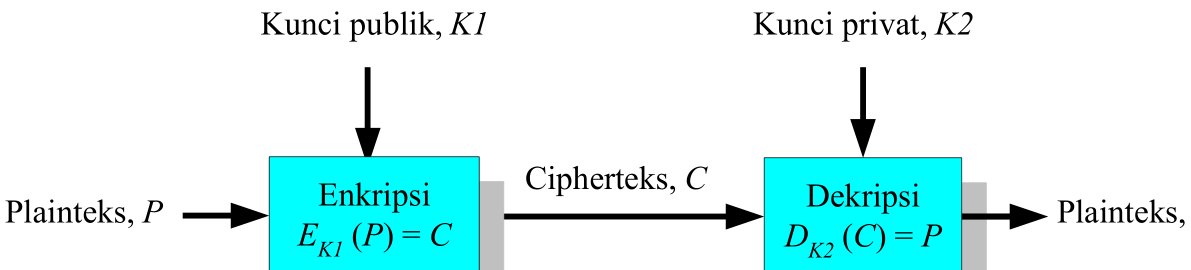
\includegraphics[width=130.20mm,height=74.25mm]{../../images/llm/page_060_img_01.png}%
\end{textblock*}

\end{document}
